\subsection{Comparison of Models}

The purpose of this work serves to provide recommendations for developing a wireless network intrusion detection system, however, evaluating the performances of the models poses a challenge when determining the 'best' model for each algorithm. Challenges arise when multiple metrics and performance indicators are to be compared. The analysis focused on achieving a balance between avoiding false positives (instances where normal traffic is marked as malicious) and false negatives (instances of malicious traffic marked as normal). The aim was to identify a model that was capable of distinguishing between the 6 attack classes and avoiding as many false negatives and positives as possible. The following sections compare the three 'best' identified models from the following models: Random Forest, XGBoost and Multi-Layer Perceptron (MLP).

\subsubsection*{Random Forest}

During experimentation, several Random Forest models were trained, and attempts were made to search through a series of parameters, using the evaluation metrics defined previously, Model ID 1 displayed strong consistent performance during CV and testing. It achieved an AUC of 99.99, F1 of 99.66, Precision of 99.66, Recall of 99.67 and Accuracy of 99.67 on the test set, indicating that it was able to correctly classify the six attack classes with a high degree of accuracy. The model's confusion matrix shows a good balance between FP and FNs on majority classes, whilst it did struggle slightly on Botnet and SSH, the total number of misclassification remained relatively low. \ref{tab:rf_class_report}, \ref{fig:rf_model1_cm} and \ref{fig:rf_model1_fi} show the Classification, Confusion Matrix and Feature Importances for the model.

\begin{table}[htbp]
  \centering
  \caption{RF Model 1 Classification Report}
  \label{tab:rf_class_report}
    \begin{tabular}{lcccc}
    \toprule
    Class & Precision & Recall & F1-Score & Support \\
    \midrule
    Botnet & 0.95 & {\color{red}\bfseries 0.77} & {\color{red}\bfseries 0.85} & 17060 \\
    Malware & {\color{red}\bfseries 0.89} & 0.82 & 0.86 & 39476 \\
    Normal & 1.00 & 1.00 & 1.00 & 4572206 \\
    SQL Injection & 0.93 & 0.86 & 0.89 & 789 \\
    SSDP & 1.00 & 1.00 & 1.00 & 1649955 \\
    SSH & 0.94 & 0.79 & 0.86 & 3565 \\
    Website Spoofing & 0.99 & 0.98 & 0.98 & 121533 \\
    \midrule
    Accuracy & & & 1.00 & 6404584 \\
    Macro Avg & 0.96 & 0.89 & 0.92 & 6404584 \\
    Weighted Avg & 1.00 & 1.00 & 1.00 & 6404584 \\
    \bottomrule
    \end{tabular}
\end{table}

\begin{figure}[H]
    \centering
	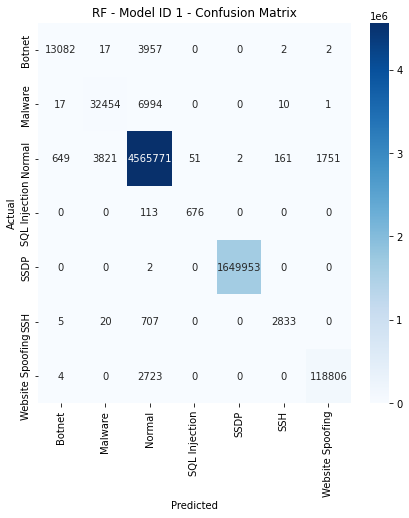
\includegraphics[width=0.8\textwidth]{Appendices/Images/RF/Model1/RF_Model1_CM.png}
	\caption{RF Model 1 CM}
  	\label{fig:rf_model1_cm}
\end{figure}

\begin{figure}[H]
    \centering
	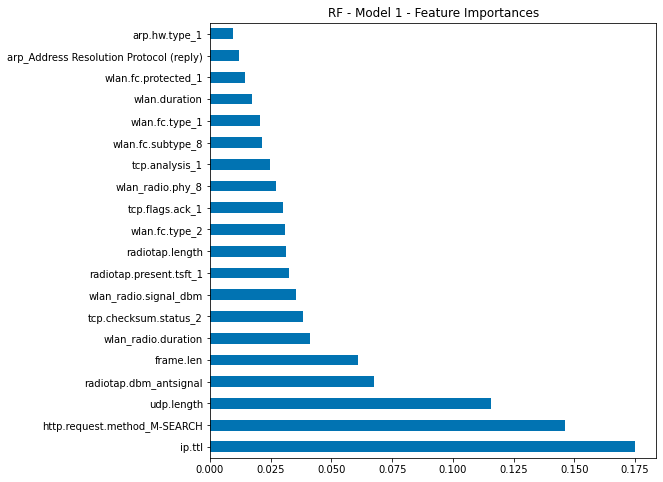
\includegraphics[width=\textwidth]{Appendices/Images/RF/Model1/RF_Model1_FI.png}
	\caption{RF Model 1 FI}
  	\label{fig:rf_model1_fi}
\end{figure}


\subsubsection*{XGBoost}

Comparing all 11 models trained on the XGBoost Classifier, Model 10 achieved superiority with an AUC of 99.99 (rounding to 100), F1 of 99.65, Precision of 99.65, Recall of 99.66 and Accuracy of 99.66 across the test set and similar during Cross Validated training.  

%% TODO XGBOOST Best Model

\begin{table}[htbp]
  \centering
  \caption{XGBoost Best Model Classification Report}
  \label{tab:xgb_class_report}
    \begin{tabular}{lcccc}
    \toprule
    Class & Precision & Recall & F1-Score & Support \\
    \midrule
    Botnet & 0.96 & 0.75 & {\color{red}\bfseries 0.84} & 17060 \\
    Malware & {\color{red}\bfseries 0.89} & 0.82 & 0.85 & 39476 \\
    Normal & 1.00 & 1.00 & 1.00 & 4572206 \\
    SQL Injection & 0.94 & 0.89 & {\color{red}\bfseries 0.91} & 789 \\
    SSDP & 1.00 & 1.00 & 1.00 & 1649955 \\
    SSH & 0.92 & {\color{red}\bfseries 0.78} & 0.85 & 3565 \\
    Website Spoofing & 0.99 & 0.97 & 0.98 & 121533 \\
    \midrule
    Accuracy & & & 0.99 & 6404584 \\
    Macro Avg & 0.83 & 0.73 & 0.80 & 6404584 \\
    Weighted Avg & 0.99 & 0.99 & 0.99 & 6404584 \\
    \bottomrule
    \end{tabular}
\end{table}

\begin{figure}[H]
	\centering
	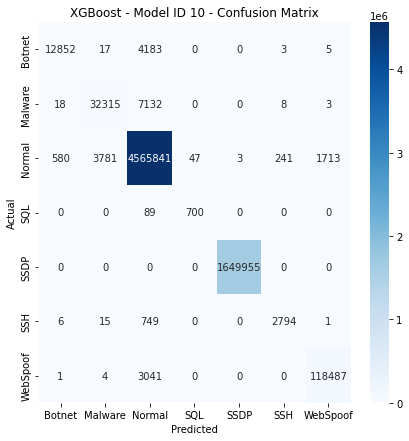
\includegraphics[width=0.8\textwidth]{Appendices/Images/XGB/Model10/XGB_Model10_CM.png}
	\caption{XGBoost Model 10 CM}
  	\label{fig:xgb_model10_cm}
\end{figure}

\begin{figure}[H]
	\centering
	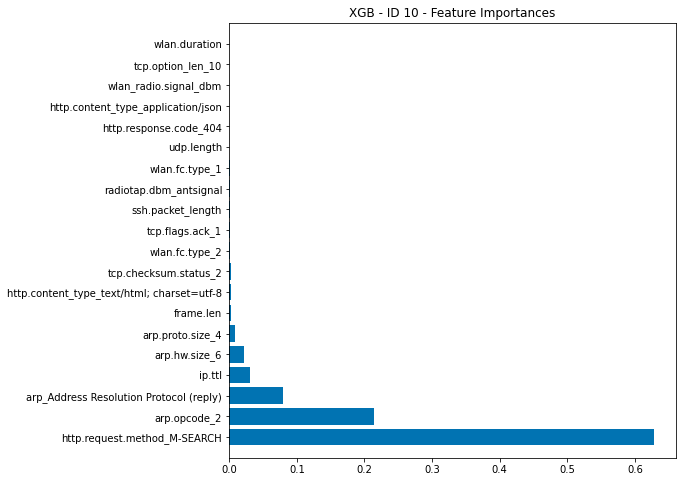
\includegraphics[width=\textwidth]{Appendices/Images/XGB/Model10/XGB_Model10_FI.png}
	\caption{XGBoost Model10 Feature Importance}
  	\label{fig:xgb_model10_fi}
\end{figure}


% MLP
\subsubsection*{MLP}

Out of all models trained, model 4 showed strong performance overall with a good proportion of instances from classes Botnet, Malware, Normal and SDDP being accurately classified. While the model struggles with SQL Injection and SSH with poor recall and F1 scores, this was expected given the imbalance in the dataset. Metrics were consistent across S-CV and the test set, indicating that the MLP model was not overfitting the training data and generalising well on new unseen data. Table \ref{tab:mlp_class_report} and \ref{fig:mlp_model4_cm} shows the Classification Report and Confusion Matrix for the model. 

\begin{table}[htbp]
  \centering
  \caption{MLP Best Model Classification Report}
  \label{tab:mlp_class_report}
    \begin{tabular}{lcccc}
    \toprule
    Class & Precision & Recall & F1-Score & Support \\
    \midrule
    Botnet & 0.94 & 0.61 & 0.74 & 17060 \\
    Malware & 0.89 & 0.72 & 0.80 & 39476 \\
    Normal & 0.99 & 1.00 & 1.00 & 4572206 \\
    SQL Injection & 0.99 & {\color{red}\bfseries 0.37} & {\color{red}\bfseries 0.54} & 789 \\
    SSDP & 1.00 & 1.00 & 1.00 & 1649955 \\
    SSH & {\color{red}\bfseries 0.83} & 0.48 & 0.60 & 3565 \\
    Website Spoofing & 1.00 & 0.92 & 0.95 & 121533 \\
    \midrule
    Accuracy & & & 0.99 & 6404584 \\
    Macro Avg & 0.83 & 0.73 & 0.80 & 6404584 \\
    Weighted Avg & 0.99 & 0.99 & 0.99 & 6404584 \\
    \bottomrule
    \end{tabular}
\end{table}

\begin{figure}[H]
    \centering
	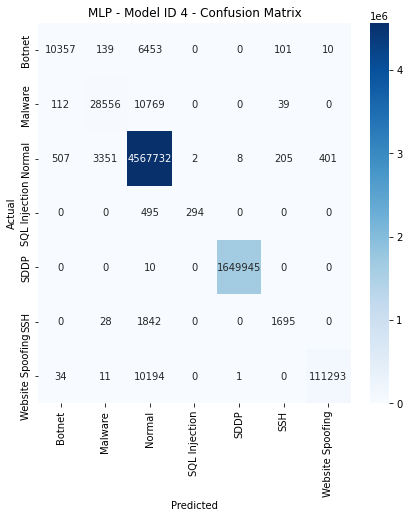
\includegraphics[width=0.8\textwidth]{Appendices/Images/MLP/MLP_Model4_CM.png}
	\caption{MLP Model 4 CM}
  	\label{fig:mlp_model4_cm}
\end{figure}

\subsection{Limitations}

The experiments faced several limitations that should be considered in the interpretation of results and impact findings in this dissertation. 

Firstly, the constraints of time and computational resources hindered the ability to construct and test an exhaustive list of models and the frequent occurrence of hardware and OS crashes negatively disrupted model training, leading to a loss in progress. 
GridSearchCV is a searching method used to find optimal parameters, it was not utilised to the full extent due to similar constraints, which meant models were not tuned exhaustively, possibly leading to lower performance.

Lastly, the iterative and exploratory approach taken for model selection and tuning could be a source of error. This may have been susceptible to undue bias or randomness, potentially leading to under-explored models. 

These limitations prove that although the results are high, consideration should be exercised with caution with evaluating their use for a proposed IDS. Additional research is needed to validate these models and further work is suggested to investigate other, more complex and tuned models.

\subsection{Recommendations}

Comparing all three machine learning algorithms, experiments from this study show that the Random Forest model ran with default parameters displayed slightly better results compared to the other two. The XGBoost model also performed very well with similar results but had a small increase in false positives for Botnet, Malware and SSH. The MLP model, whilst still displaying high levels of performance, appeared to struggle with the classification of minority classes. The Confusion matrix contains a high number of false negatives for Botnet, Malware and SSH, suggesting it was unable to accurately predict these classes.

As mentioned, identifying the most optimal solution for a proposed Wireless Network Intrusion Detection System is a highly subjective challenge. The final decision hinges on the performance of the models within the author's environment and ultimately depends on the particular needs and focuses in the production environment. 